\begin{flushright} {\tiny {\color{gray} (tikz\_4x3x2\_q2.tex)}} \end{flushright}
%~~~~~~~~~~~~~~~~~~~~~~~~~~~~~~~~~~~~~~~~~~~~~~~~~~~~~~~~~~~~~~~~~~~~~~~~~~~~~~~~~~~~~~~~~~~~~~~~~~

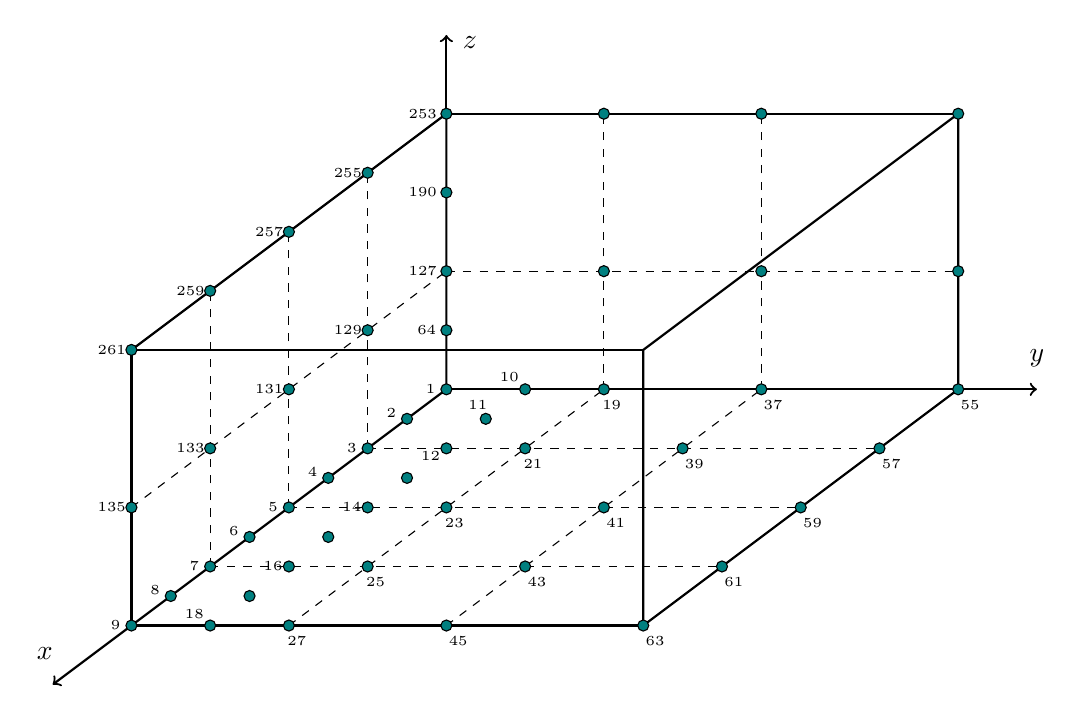
\begin{tikzpicture}
%\draw[step=0.5cm,gray,very thin] (0,0) grid (14,10); %background grid

%element
\draw[thick] (2,2) -- (8.5,2) -- (8.5,5.5) -- (2,5.5) -- cycle;  
\draw[thick] (2,2) -- (6,5) -- (6,8.5) -- (2,5.5) -- cycle ;
\draw[thick] (8.5,2) -- (12.5,5) -- (12.5,8.5) -- (8.5,5.5) -- cycle ;
\draw[thick] (6,5) -- (12.5,5) ;
\draw[thick] (6,8.5) -- (12.5,8.5) ;

%axes
\draw[thick,->] (2,2)--(1,1.25);
\draw[thick,->] (12.5,5)--(13.5,5);
\draw[thick,->] (6,8.5)--(6,9.5);
\node[] at (0.9,1.65) {$x$};
\node[] at (13.5,5.4) {$y$};
\node[] at (6.3,9.4) {$z$};

\draw[dashed] (2,3.5)--(6,6.5);
\draw[dashed] (3,2.75)--(3,6.25);
\draw[dashed] (4,3.5)--(4,7);
\draw[dashed] (5,4.25)--(5,7.75);
\draw[dashed] (4,2)--(8,5);
\draw[dashed] (6,2)--(10,5);
\draw[dashed] (3,2.75)--(9.5,2.75);
\draw[dashed] (4,3.5)--(10.5,3.5);
\draw[dashed] (5,4.25)--(11.5,4.25);
\draw[dashed] (6,6.5)--(12.5,6.5);
\draw[dashed] (8,5)--(8,8.5);
\draw[dashed] (10,5)--(10,8.5);


\draw[black,fill=teal] (2,2) circle (2pt);  %9
\draw[black,fill=teal] (2.5,2.375) circle (2pt); 
\draw[black,fill=teal] (3,2.75) circle (2pt); 
\draw[black,fill=teal] (3.5,3.125) circle (2pt); 
\draw[black,fill=teal] (4,3.5) circle (2pt); 
\draw[black,fill=teal] (4.5,3.875) circle (2pt); 
\draw[black,fill=teal] (5,4.25) circle (2pt); 
\draw[black,fill=teal] (5.5,4.625) circle (2pt); 
\draw[black,fill=teal] (6,5) circle (2pt);  % 1

\draw[black,fill=teal] (3,2) circle (2pt);  %18
\draw[black,fill=teal] (3.5,2.375) circle (2pt); 
\draw[black,fill=teal] (4,2.75) circle (2pt); 
\draw[black,fill=teal] (4.5,3.125) circle (2pt); 
\draw[black,fill=teal] (5,3.5) circle (2pt); 
\draw[black,fill=teal] (5.5,3.875) circle (2pt); 
\draw[black,fill=teal] (6,4.25) circle (2pt); 
\draw[black,fill=teal] (6.5,4.625) circle (2pt); 
\draw[black,fill=teal] (7,5) circle (2pt);  % 10



\draw[black,fill=teal] (2,3.5) circle (2pt); 
\draw[black,fill=teal] (3,4.25) circle (2pt); 
\draw[black,fill=teal] (4,5) circle (2pt); 
\draw[black,fill=teal] (5,5.75) circle (2pt); 
\draw[black,fill=teal] (6,6.5) circle (2pt); 

\draw[black,fill=teal] (2,5.5) circle (2pt); 
\draw[black,fill=teal] (3,6.25) circle (2pt); 
\draw[black,fill=teal] (4,7) circle (2pt); 
\draw[black,fill=teal] (5,7.75) circle (2pt); 
\draw[black,fill=teal] (6,8.5) circle (2pt); 

\draw[black,fill=teal] (4,2) circle (2pt); 
\draw[black,fill=teal] (5,2.75) circle (2pt); 
\draw[black,fill=teal] (6,3.5) circle (2pt); 
\draw[black,fill=teal] (7,4.25) circle (2pt); 
\draw[black,fill=teal] (8,5) circle (2pt); 

\draw[black,fill=teal] (6,2) circle (2pt); 
\draw[black,fill=teal] (7,2.75) circle (2pt); 
\draw[black,fill=teal] (8,3.5) circle (2pt); 
\draw[black,fill=teal] (9,4.25) circle (2pt); 
\draw[black,fill=teal] (10,5) circle (2pt); 

\draw[black,fill=teal] (8.5,2) circle (2pt); 
\draw[black,fill=teal] (9.5,2.75) circle (2pt); 
\draw[black,fill=teal] (10.5,3.5) circle (2pt); 
\draw[black,fill=teal] (11.5,4.25) circle (2pt); 
\draw[black,fill=teal] (12.5,5) circle (2pt);

\draw[black,fill=teal] (6,5.75) circle (2pt); %64
\draw[black,fill=teal] (6,7.5) circle (2pt); %190

\draw[black,fill=teal] (8,6.5) circle (2pt);
\draw[black,fill=teal] (8,8.5) circle (2pt);

\draw[black,fill=teal] (10,6.5) circle (2pt);
\draw[black,fill=teal] (10,8.5) circle (2pt);

\draw[black,fill=teal] (12.5,6.5) circle (2pt);
\draw[black,fill=teal] (12.5,8.5) circle (2pt);

\node[] at (5.8,5) {\tiny 1};
\node[] at (5.3,4.7) {\tiny 2};
\node[] at (4.8,4.25) {\tiny 3};
\node[] at (4.3,3.95) {\tiny 4};
\node[] at (3.8,3.5) {\tiny 5};
\node[] at (3.3,3.2) {\tiny 6};
\node[] at (2.8,2.75) {\tiny 7};
\node[] at (2.3,2.45) {\tiny 8};
\node[] at (1.8,2) {\tiny 9};

\node[] at (6.8,5.15) {\tiny 10};
\node[] at (6.4,4.8) {\tiny 11};
\node[] at (5.8,4.15) {\tiny 12};
\node[] at (4.8,3.5) {\tiny 14};
\node[] at (3.8,2.75) {\tiny 16};
\node[] at (2.8,2.15) {\tiny 18};

\node[] at (8.1,4.8) {\tiny 19};
\node[] at (7.1,4.05) {\tiny 21};
\node[] at (6.1,3.3) {\tiny 23};
\node[] at (5.1,2.55) {\tiny 25};
\node[] at (4.1,1.8) {\tiny 27};

\node[] at (10.15,4.8) {\tiny 37};
\node[] at (9.15,4.05) {\tiny 39};
\node[] at (8.15,3.3) {\tiny 41};
\node[] at (7.15,2.55) {\tiny 43};
\node[] at (6.15,1.8) {\tiny 45};

\node[] at (12.65,4.8) {\tiny 55};
\node[] at (11.65,4.05) {\tiny 57};
\node[] at (10.65,3.3) {\tiny 59};
\node[] at (9.65,2.55) {\tiny 61};
\node[] at (8.65,1.8) {\tiny 63};

\node[] at (5.75,5.75) {\tiny 64};

\node[] at (5.7,6.5) {\tiny 127};
\node[] at (4.75,5.75) {\tiny 129};
\node[] at (3.75,5) {\tiny 131};
\node[] at (2.75,4.25) {\tiny 133};
\node[] at (1.75,3.5) {\tiny 135};

\node[] at (5.7,7.5) {\tiny 190};

\node[] at (5.7,8.5) {\tiny 253};
\node[] at (4.75,7.75) {\tiny 255};
\node[] at (3.75,7) {\tiny 257};
\node[] at (2.75,6.25) {\tiny 259};
\node[] at (1.75,5.5) {\tiny 261};

\end{tikzpicture}

